\documentclass[acmlarge]{acmart}

\usepackage{booktabs} % For formal tables


\usepackage[ruled]{algorithm2e} % For algorithms
\usepackage{graphicx}
\usepackage{tabu}
\usepackage{float}
\graphicspath{{images/}}

%\renewcommand{\algorithmcfname}{ALGORITHM}
%\SetAlFnt{\small}
%\SetAlCapFnt{\small}
%\SetAlCapNameFnt{\small}
%\SetAlCapHSkip{0pt}
\IncMargin{-\parindent}


% Metadata Information
%\acmJournal{POMACS}
%\acmVolume{9}
%\acmNumber{4}
%\acmArticle{39}
\acmYear{2017}
\acmMonth{5}
%\acmArticleSeq{11}

%\acmBadgeR[http://ctuning.org/ae/ppopp2016.html]{ae-logo}
%\acmBadgeL[http://ctuning.org/ae/ppopp2016.html]{ae-logo}


% Copyright
%\setcopyright{acmcopyright}
%\setcopyright{acmlicensed}
%\setcopyright{rightsretained}
%\setcopyright{usgov}
%\setcopyright{usgovmixed}
%\setcopyright{cagov}
%\setcopyright{cagovmixed}

% DOI
%\acmDOI{0000001.0000001}

% Paper history
%\received{February 2007}
%\received{March 2009}
%\received[accepted]{June 2009}


% Document starts
\begin{document}
% Title portion
\title{Performance Comparison of a DNA based Cryptosystem and Modern Cryptosystems} 
\author{Paul Emil Ongoco}
\affiliation{%
  \institution{University of the Philippines Diliman}
  \city{Quezon City}
  \country{Philippines}}
\author{Patrick Angelo Roderno}
\affiliation{%
  \institution{University of the Philippines Diliman}
  \city{Quezon City}
  \country{Philippines}
}


\begin{abstract}
As computers become more powerful, existing cryptosystems become vulnerable to attacks. This trend caused a nonstop attempt to improve security. Since the emergence of DNA computation, researches have focused in exploring its potential applications in cryptography due to its massive parallelism and high-density information storage. Since DNA cryptography is relatively new, the existing proposals for DNA-based cryptosystems are mainly theoretical and are still to be used in real life applications. We are developing a new and improved DNA-based cryptosystem based on an existing one. Comparative study to other modern cryptosystems (AES, etc.) will be done to determine if the new cryptosystem meet the standards of today's cryptography. Our results show that adding a layer of security through a steganographic approach proved to be impractical because of its time complexity of $O(n^2)$. This is due to the generation of random strands of DNA used to hide the ciphertext. 
\end{abstract}


%
% The code below should be generated by the tool at
% http://dl.acm.org/ccs.cfm
% Please copy and paste the code instead of the example below. 
%
\begin{CCSXML}
<ccs2012>
    <concept>
        <concept_id>10002978.10002979.10002982.10011598</concept_id>
        <concept_desc>Security and privacy~Block and stream ciphers</concept_desc>
        <concept_significance>500</concept_significance>
    </concept>
    <concept>
        <concept_id>10002978.10002979.10002984</concept_id>
        <concept_desc>Security and privacy~Information-theoretic techniques</concept_desc>
        <concept_significance>300</concept_significance>
    </concept>
</ccs2012>
\end{CCSXML}

\ccsdesc[500]{Security and privacy~Block and stream ciphers}
\ccsdesc[300]{Security and privacy~Information-theoretic techniques}

%
% End generated code
%


\keywords{DNA cryptosystem, RSA, Advanced Encryption Scheme, Triple DES, Steganography, DNA computer, Nitrogenous bases,}


%\thanks{This work is supported by the National Science Foundation,
%  under grant CNS-0435060, grant CCR-0325197 and grant EN-CS-0329609.

%  Author's addresses: G. Zhou, Computer Science Department, College of
%  William and Mary; Y. Wu {and} J. A. Stankovic, Computer Science
%  Department, University of Virginia; T. Yan, Eaton Innovation Center;
%  T. He, Computer Science Department, University of Minnesota; C.
%  Huang, Google; T. F. Abdelzaher, (Current address) NASA Ames
%  Research Center, Moffett Field, California 94035.}


\maketitle

% The default list of authors is too long for headers}
%\renewcommand{\shortauthors}{G. Zhou et al.}

\section{Introduction}

Through the years of development of computer technology, security has always been an issue. As computers become more and more powerful, they also become more capable of breaking cryptosystems. This means that there is a continuous need to improve or develop new and reliable cryptosystems. In 1994, computer scientist Leonard Adleman introduced DNA computing in his paper titled "Computing with DNA" where he presented how he used DNA to solve a Hamiltonian Path Problem \cite{adleman}. His invention opened a lot of new opportunities in a lot of fields, and one led to DNA Cryptography.

DNA Cryptography deals with exploring the potential of the DNA's massive parallelism and information density for cryptographic purposes. It has been used to break the Data Encryption Standard (DES) \cite{dna-computing}, for steganography, authentication, and also new DNA-based cryptosystems. Although there has been a lot of research under this field, DNA Cryptography still isn't mature enough to be applied in solving real-world problems. The project is an attempt to further study the application of DNA computing in cryptography by studying an existing DNA-based cryptosystem and utilizing opportunities to improve it.

\section{Related Work}

The following section consists of background information about cryptology, modern techniques of cryptography, and performance metrics for cryptosystems. It also provides information related to DNA cryptography, including definitions and concepts about DNA and DNA computing. It discusses the pros and cons of DNA computing, the motivation behind DNA cryptography.

\subsection{Cryptology}

Cryptology is a branch of mathematics that is divided into two branches: cryptography and cryptanalysis. Cryptography is the art and science of encrypting plaintexts while cryptanalysis is the art and science of decrypting ciphertexts. Cryptology is different from other academic disciplines as there is a need for continuous interactions between cryptography and cryptanalysis for its development. Cryptographers (practitioners of cryptography) starts the interaction with the presentation of a new algorithm design, while cryptanalysts (practitioners of cryptanalysis) tries to expose the flaws of the algorithm. This creates a healthy and competitive cycle that produces "strong" cryptosystem \cite{metrics}.

\subsection{Modern Techniques of Cryptography}

This section introduces some of today's most secure cryptosystems and discuss the algorithm behind them. The cryptosystems to be discussed are Triple Data Encryption Algorithm (TDEA), Advanced Encryption Standard (AES) and Rivest-Shamir-Adleman (RSA).

\subsubsection{Triple Data Encryption Algorithm (TDEA)}

Triple Data Encryption Algorithm (TDEA) is an algorithm that consists of three DES encryptions with different keys. The DES algorithm is a symmetric cipher that encrypts blocks of size 64 bits and uses keys with size 56 bits.

The process of encryption involves 16 rounds of encryption to produce the ciphertext. Each round uses different subkey derived from the main key. After performing a bitwise permutation on the plaintext, the 64 bits of the plaintext is split into 32-bit halves ${L_i}$ and ${R_i}$ \cite{153}. In each round of the encryption, 

\begin{itemize}
    \item ${R_i}$ is fed into the function f (which uses a key ${k_i}$ derived from the original key k)
    \item Output is XORed with ${L_i}$
    \item Left and right halves are swapped.
\end{itemize}

The rounds can be expressed as, 
\begin{itemize}
    \item ${L_i}$ = ${R_{i-1}}$
    \item ${R_i}$ = ${L_{i-1}}$ XOR ${f(R_{i-1}, k_i)}$ 
\end{itemize}
    
After the 16th round, the left and right halves are then again swapped to finally make the ciphertext \cite{153}.

Nowadays, DES is easily breakable with modern computers. TDEA aims to extend the key length of the cipher to 168 bits. However, Meet-in-the-Middle attack reduces the effective key length of TDEA to 112 bits. As of today, no practical attack has been discovered that can break TDEA \cite{153}.

\begin{figure}[H]
    \centering
    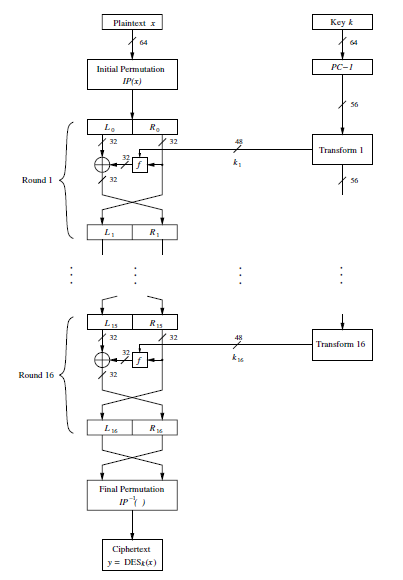
\includegraphics[width=10cm]{des_structure}
    \caption{DES Structure \cite{153}}
    \label{fig:des}
\end{figure}

\begin{figure}[H]
    \centering
    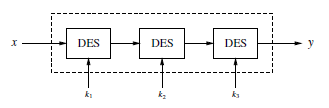
\includegraphics[width=10cm]{tdea_structure}
    \caption{TDEA Structure \cite{153}}
    \label{fig:tdea}
\end{figure}

\subsubsection{Advanced Encryption Standard (AES)}

Advanced Encryption Standard (AES) is the most used symmetric cipher today. It encrypts blocks of size 128 bits and uses keys with size 128/192/256 bits. The number of encryption rounds depends on the size of the key. 128-bit keys are used to perform 10 rounds of encryption, 192-bit keys are used to perform 12 rounds of encryption, and 256-bit keys are used to perform 14 rounds of encryption.

\begin{figure}[H]
    \centering
    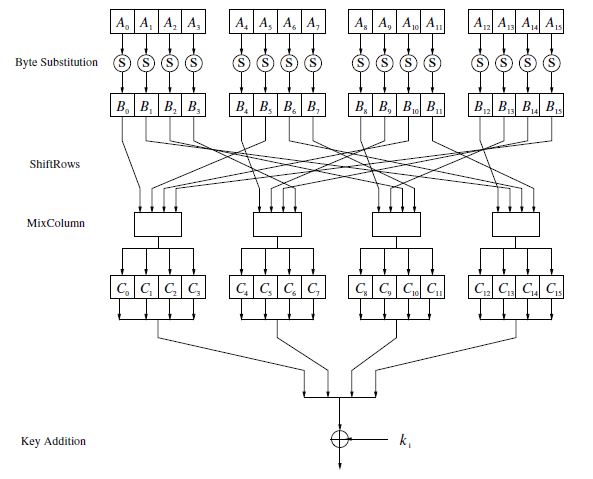
\includegraphics[width=10cm]{aes_structure}
    \caption{AES Structure \cite{153}}
    \label{fig:aes}
\end{figure}

To perform the encryption, the 128-bit data path is arranged into a 4x4 matrix, resulting into a 16-byte input. The 16-byte input will then go through several rounds of encryption composed of "layers", namely the byte substitution layer, diffusion layer, and key addition layer. \cite{153}
\begin{itemize}
    \item Byte Addition Layer: The 16-byte input is fed byte-wise into look-up tables with special mathematical properties called S-boxes. This introduces confusion to the data.
    \item Diffusion Layer: This layer provides diffusion to the data. It consists of two sublayers:
    \begin{itemize}
        \item ShiftRows sublayer: permutes the data on a byte level
        \item MixColumns sublayer: mixes blocks of four bytes
    \end{itemize}
    \item Key Addition Layer: This layer performs an XOR operation to the 16-byte input with a 128-bit round key, which has been derived from the main key in the key schedule.
\end{itemize}

\subsubsection{Rivest-Shamir-Adleman (RSA) Cryptosystem}

Rivest-Shamir-Adleman (RSA) is the most widely used asymmetric used cryptosystem today. The encryption and decryption operations of RSA are simply an exponentiation in an integer ring ${Z_n}$ where ${n = p*q}$ where p, q are large prime numbers \cite{153}.

RSA Encryption: Given the public key (n,e) = ${k_{pub}}$ and the plaintext x, the encryption function is:
\begin{center}
    ${y\ =\ e_{k_{pub}} (x)\ =\ x^e\ mod\ n}$
\end{center}
where x, y ${\epsilon}$ ${Z_n}$

RSA Decryption: Given the private key d = ${k_{pr}}$ and the ciphertext y, the decryption function is:
\begin{center}
    ${x\ =\ d_{k_{pr}} (y) =\ y^d\ mod\ n}$
\end{center}
where x, y ${\epsilon}$ ${Z_n}$ \

RSA Keypair Generation: 
\begin{enumerate}
    \item Choose two large primes p and q
    \item Compute ${n\ =\ p*q}$
    \item Compute ${\phi(n)\ =\ (p-1)*(q-1)}$
    \item Select public exponent e ${\epsilon}$ ${\{1, 2, ..., \phi(n)-1}\}$ such that ${gcd(e,\phi(n))=1}$
\end{enumerate}

Usually, x, y, n, and d are very long integer numbers, with length of 1024 bits or more. RSA is considered secure due to the fact that it is hard to derive the private key given the public key \cite{153}.

\subsection{Cryptographic Algorithm Metrics}

Norstad and Smith Jr. \cite{metrics} provided performance metrics for cryptosystems to assess the strength of cryptosystems objectively rather than subjectively. These metrics are as follows:
\begin{enumerate}
    \item Key Length Metric: The cryptographic strength of symmetric cryptosystems is a function of key length. The longer the key, the more resistant the cryptosystem is to brute force attacks.
    \item Attack Steps Metric: Number of steps required to perform the best known attack.
    \item Attack Time Metric: Time required to perform the fastest known attack on a specific processor
    \item Rounds metric: Number of rounds of encryption done in the cryptosystem
    \item Algorithm Strength Metric: This metric is measured through a list of attributes that will evaluate the strength of the system. The list includes:
    \begin{itemize}
        \item The plaintext cannot be derived from the ciphertext without a key.
        \item There should be no plaintext attack that is better than a brute force attack.
        \item Knowledge of the algorithm should not reduce the strength of the cipher.
        \item There should be no correlation between any input bits or key bits and the output bits.
        \item The algorithm should contain noncommutative combination of substitution and permutation, except for publick key algorithms.
        \item The algorithm should include substitutions and permutations
        under the influence of both the input data and the key.
        \item Redundant bit groups in the plaintext should be totally obscured in the ciphertext.
        \item The length of the ciphertext should be the same as the length of the plaintext.
        \item Any possible key should produce a strong cipher, although this is not always true for many good algorithms such as DES and most public key algorithms.
    \end{itemize}
    A scale for cryptographic strength is also given.
    \begin{itemize}
        \item Unconditionally Secure (US): A cipher is Unconditionally Secure if there is not enough information in the ciphertext to decrypt the message no matter how much ciphertext is intercepted.
        \item Computationally Secure (CS): A cipher is Computationally Secure if the cipher cannot be broken in a reasonable amount of time with the available resources.
        \item Conditionally Computationally Secure (CCS): A cipher is Conditionally Computationally Secure if the cipher could be implemented with short keys or that the cipher does not have sufficient rounds to earn the CS rating.
        \item Weak (W): A cipher is Weak if it can be broken by brute force attack such that the key can be recovered in an acceptable length of time (24 hours) with an "affordable" investment (\$200,000) in cryptanalytic resources.
        \item Very Weak (VW): A Very Weak cipher can be broken by brute force attack such that the key can be recovered in a short period of time (8 hours) with cheap investment (\$20,000) in cryptanalytic resources.
    \end{itemize}
\end{enumerate}

\subsection{Deoxyribonucleic Acid (DNA)}

Deoxyribonucleic Acid, or simply DNA, is a molecule that contains the instructions an organism needs to develop, live and reproduce. It is made up of molecules called nucleotides. Each nucleotide contains a phosphate group, a sugar group, and a nitrogen base. There are four types of nitrogen bases, namely adenine (A), thymine (T), guanine (G), and cytosine (C). The order of these bases is what determines a DNA’s instructions, or genetic code. Nucleotides are attached together to form two long strands that spiral to create a double helix form. The nitrogen bases on one strand pair with the bases on another strand: adenine pairs with thymine, and guanine pairs with cytosine \cite{dna}.

The DNA has the ability to replicate, or make copies of itself. Both strands of DNA in the double helix can serve as a template for duplicating the sequence of bases \cite{dna_ghr}. Polymerase Chain Reaction (PCR), a laboratory technique invented in the 1980s, enables the replication of a specific DNA sequence, creating millions of copies of the specific DNA within a short period of time.  To perform PCR, the following components are required:
\begin{itemize}
    \item DNA Template: Sample DNA containing the target DNA sequence
    \item DNA Polymerase: The enzyme that synthesizes fresh DNA strands complementary to the target DNA sequence
    \item Primers: Short single-stranded DNA that help DNA polymerase to synthesize new DNA strands
    \item Nucleotides: Free bases A, C, T and G that will act as raw material for new DNA synthesis
    \item Buffer (usually MgCl2): Salt solution used to stabilize the reaction components and maintain optimal pH during the reaction
    \item Deionized Water: Provides liquid environment needed for the reaction
\end{itemize}
\par
Key steps in Polymerase Chain Reaction include DNA Denaturation, Primer Annealing, and Extension of Primer. These steps are repeated multiple times for amplification of the newly synthesized DNA \cite{pcr}.

\subsection{DNA Computing}

DNA computing is a new field of study that is concerned with the use of DNA molecules as tools to perform computations. The field was initially developed by Leonard Adleman in 1994 when he successfully solved the Hamiltonian Path Problem with the use of DNA. Since then, several efforts have been made to explore the field and solve actual problems with it. For example, Lipton \cite{intractable-problems} designed a simple algorithm to solve the satisfaction problem using the concepts of DNA. Also, Ray and Ogihara \cite{logic-gates} were able to develop DNA logic gates using common laboratory methods such as DNA ligation and gel electrophoresis.

\begin{figure}[H]
    \centering
    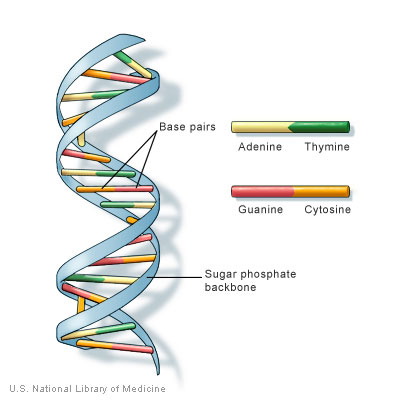
\includegraphics[width=10cm]{dna_structure}
    \caption{DNA Structure. Photo courtesy of US National Library of Medicine}
    \label{fig:dna}
\end{figure}

The operations used in DNA computing are limited to the capabilities of molecular biology. These operations are as follows \cite{processes}:
\begin{itemize}
    \item Merge: The process of combining the contents of two test tubes in a third one.
    \item Anneal: The process in which the DNA solution is cooled, causing the complementary DNA strands to pair and form the double helix structure. 
    \item Melt: Melting is the inverse process of annealing. The DNA solution is subjected to heat, causing the bonds between the double helix DNA strand to break, resulting into two single strand DNA.
    \item Separation by length: The contents of the tube are separated by increasing length using gel electrophoresis.
    \item Separation by sequence: This operation allows the removal of all DNA strands that has the desired sequence from the solution.
    \item Copying/Amplification: Copies of a specific DNA sequence is synthesized in a test tube. The start and end sequences, also known as primers, of the specific DNA sequence is needed for the amplification.
    \item Detect: The process which determines whether or not a test tube contains at least one DNA strand.
\end{itemize}

The motivation behind DNA computing is the innate characteristics of the DNA. It exhibits high performance rate, massive parallelism, and extremely high information density. In these fields, DNA is superior even to modern computers. However, it suffers from several drawbacks which makes it inapplicable to real-world problems. Generating solution sets for even simple problems may require impractically large amounts of memory. DNA synthesis is also susceptible to errors, such as mismatching pairs, and high dependency on the accuracy of the enzymes. Lastly, since a set of DNA strands is only suited for a specific problem, a brand new set would have to be made for each problem \cite{eval}.

\subsection{DNA Cryptography}

DNA Cryptography is the application of DNA computing to the field of information security. It deals with exploring the potential of DNA's large scale parallel processing and information density for cryptographic purposes. Initial accomplishments in the field include breaking traditional cryptosystems like Data Encryption Scheme (DES) and RSA, and encryption schemes that uses one-time pads and steganography \cite{dna-computing}. Although there has been a lot of research under this field, DNA Cryptography is still not mature enough to be applied in solving real-world problems because of the disadvantages of DNA computing \cite{eval}.

The security of the existing cryptosystems heavily relies on the complexity of mathematical problems. As computers become more capable of handling more complex operations, these cryptosystems become vulnerable. In 1994, when Leonard Adleman introduced DNA computing, it quickly became one of the focus of research in the field of cryptography. Computer scientists aim to harness the DNA's massive parallelism and be able to create a DNA-based cryptosystem that is more reliable and efficient than what exists now. Some of the many efforts of researchers are discussed below.

In his paper, Chen designed a cryptosystem that uses carbon nanotubes to transform data between DNA and conventional binary storage media \cite{c-nanotubes}. He assumed that the inputs to the cryptosystem are short plaintext messages, and performs modulo-2 addition operation method to encrypt large numbers of plain text using one-time-pads. One-time-pads are keys that are made randomly and used only once. Chen was also able to encode a two-dimensional picture with his design. However, one-time-pad encryption is impractical since the key can only be used once and it has to be as long as the plaintext message itself which makes it undesirable in real world situations specially in systems that uses long and varying plaintexts.

Fasila et al. presented a new hybrid cryptosystem that uses Red, Green, and Blue (RGB) colors to further improve the security of data. The cryptosystem combines a data encryption mechanism where the data is transformed into a matrix, perform matrix manipulation steps on it, encrypt it to full DNA sequence form, then use a key encapsulation scheme that uses DNA steganography \cite{fasila-system}. Ultimately, the cryptosystem is a symmetric cryptosystem thus, may suffer from the common vulnerabilities of such cryptosystems. For example, if an attacker acquired the key used in encrypting a message, it will allow him to decrypt the message. Also, the matrix manipulation is performed 2n times, where n is the length of the initial key. A long key would make the data more secure, but will make it impractical due to performance and resource limitations.

Leier et al. proposed two approaches in cryptography that makes use of DNA binary strands. The first approach uses the DNA binary strands in steganography, a technique in encryption by information hiding. The second approach uses the method of graphical subtraction and binary gel images to constitute a molecular checksum. DNA binary strands are assembled by concatenation of short double stranded DNA molecules that represents 0 (0-DNA bit), 1 (1-DNA bit), and start and end primers \cite{leier}.

In the paper of Thiruthuvadoss \cite{mastersangeline}, she describes a DNA-based cryptosystem that uses one-time pads (OTP) for encryption, collected from the gene database of the National Center for Biotechnology Information (NCBI), and Diffie-Hellman Key Exchange to enable the receiver to accurately look for the OTP. Decryption is done by reversing the encryption process (Symmetric). In her example, she used a plaintext, converted into ascii, then converted it to a binary message before encryption. The length of an encrypted message depends on how many binary 1-bit present in the binary message instead of the usual twice as long as the unencrypted message.

\section{Problem Statement}

DNA-based cryptography has been one of the focuses of research in computer security since the introduction of DNA computing by Leonard Adleman.  The technology is promising as it takes advantage of the DNA's extreme parallelism in computing and it's density when it comes to information storage. However, no existing DNA-based cryptosystem can be used in a large-scale basis due to practicality. In line with this, we are developing a new and improved DNA-based cryptosystem based on another DNA-based cryptosystem. We will also conduct a comparative study of the new DNA-based cryptosystem to other similar cryptosystems, including the cryptosystem in which the new cryptosystem is based from, in order to contribute to the realization of practical DNA-based cryptosystems. A comparative study will help in determining the weaknesses of the cryptosystems, allowing researchers to revise them to address these weaknesses.

Note that the study is limited to simulations of the cryptosystems in a computer rather than performing an actual experiment on a molecular biology laboratory due to the inaccessibility of such laboratories.

\section{Methodology}
In the beginning of this study, the researchers selected the first method of DNA steganography proposed and described in the paper "Cryptography with DNA binary strands" by Leier et al\cite{leier}. The method is simulated using the programming language Python 2.7 following the same algorithm as described in the said paper.

\subsection{DNA Steganography}
\subsubsection{Plaintext to DNA}
A string from an input file serves as the plaintext message. First, the string is converted into binary format where each character in the message becomes an 8-bit binary of their corresponding ASCII value. After acquiring the binary form of the plaintext, it can be further converted to a DNA strand format by arbitrarily assigning 2-bit binary to each of the nitrogenous bases e.g. "A" is 01, "C" is 00, "T" is 11, and "G" is 10. From the acquired DNA strand form of the plaintext, we select start and end primers to be used as keys for decryption. In this case, they are first one-fifth (in terms of length) and the complement of the last one-fifth of the plaintext in DNA form.

\subsubsection{Generation of random DNA strands}
In order to perform Steganography, the plaintext in DNA strand form must be hidden within other random DNA strands as if to hide it's existence i.e. extremely low chance of being able to randomly select it from the set of all DNA strands. In a molecular biology laboratory, this is done by mixing the plaintext DNA strand with random strands of DNA or nitrogenous bases thus hiding it among billions of other DNA strands. In this simulation, the DNA strands are randomly generated and are randomly placed in a file together with the message DNA and the primers. The randomly generated DNA strands have the same length as the message DNA. This step can be considered as the "encryption" process and its security is directly proportional to the amount of randomly generated DNA strands.

\subsubsection{Decryption}
The decryption is mainly done by the process of Polymerase Chain Reaction. The idea is to duplicate the desired strand repeatedly to the point that you are certain such that if you randomly choose a strand from the set, what you get is the strand containing the message. To do this in the computer, scan through each strand in the set while checking if they have starts and ends that would attach to the primers we selected. The matching strands are duplicated by doubling their instances in the set. In order to acquire the message strand, randomly select from the final set of DNA strands.\\

It is not efficient to simulate PCR. This is due to the exponential increase in amount of the strands that are being processed and the fact that this whole process can just be replaced by a search function. In order to proceed with the study, a different, more "computer-friendly" DNA-based cryptosystem is selected. The cryptosystem described by Thiruthuvadoss in her paper "Comparison and Performance Evaluation of Modern Cryptography and DNA Cryptography" can be simulated in the computer without having to simulate PCR.

\subsection{DNA-based Encryption with Steganography}
\subsubsection{Plaintext to binary}
The same way it was done before, the string from an input file is converted to binary format. Each character in the string is converted to an 8-bit binary representation of their ASCII value.
\subsubsection{Encryption}
The encryption is done almost similar to what was described in the paper of Thiruthuvadoss but the key is randomly generated rather than pulled from an online database. The key used in this system is a one-time pad (OTP) in the form of a DNA strand which is ten times the length of the binary message. To encrypt the binary message, traverse through the binary message from the most significant bit to the least significant bit and the OTP from the last ten nitrogenous bases to the first 10 nitrogenous bases. If the current bit is 1, add the complement of the current ten nitrogenous bases to the ciphertext string, otherwise, traverse to the next bit and the next ten nitrogenous bases. This is done until the whole binary message is traversed. Next, generate random start and end primers with 20 nitrogenous bases and affix them accordingly to the ciphertext. This process is demonstrated in the following short example that only uses 3 nitrogenous bases for each bit instead of 10:
\begin{quote}
\textbf{Binary message:} 101\\
\textbf{OTP:} CGA ACT CCG\\
\\
Current bit: 1\\
Current OTP: CCG\\
Ciphertext: GGC\\
\\
Current bit: 0 (skip)\\
Current OTP: ACT\\
Ciphertext: GGC\\
\\
Current bit: 1\\
Current OTP: CGA\\
Ciphertext: GGC GCT\\
\\
Start Primer: ACA (arbitrary)\\
End Primer: TCG (arbitrary)\\
Ciphertext: ACA GGC GCT TCG\\
\\
END
\end{quote}
\subsubsection{Steganography}
In this step, a very long strand of DNA is created by affixing random DNA strands of varying length before and after the primers arbitrarily. This is done multiple times until the number of nitrogenous bases in the strand exceeds 3 million. This way, messages of different lengths will have the same overall length of ciphertext thus contributing to the property of steganography about hiding the existence of exclusive conversation.

\subsubsection{Decryption}
The decryption is done by searching for the primers within the long strand of DNA and getting the message strand in between them. Knowing what the primers are and how long the original ciphertext is allows us to accurately search for the desired message strand. The DNA strand within the long DNA ciphertext that begins with the start primer, ends with the end primer, and has the length of the original ciphertext is the desired strand. To extract the message, truncate the extracted strand by removing the two primers at both ends, then perform the reverse encryption process. Here, the previous example is decrypted:
\begin{quote}
\textbf{Extracted strand:} ACA GGC GCT TCG\\
\textbf{Truncated strand:} GGC GCT\\
\textbf{OTP:} CGA ACT CCG\\
\\
Current 3-base strand: GGC\\
Current OTP: CCG (complement)\\
Binary message: 1\\
\\
Current 3-base strand: GCT\\
Current OTP: ACT (not complement)\\
Binary message: 10\\
\\
Current 3-base strand: GCT\\
Current OTP: CGA (complement)\\
Binary message: 101\\
\\
END
\end{quote}

\subsection{Testing and Comparison}
The new cryptosystem is compared with the original cryptosystem by Thiruthuvadoss and the following modern cryptosystems:
\begin{itemize}
    \item Triple Data Encryption Algorithm (TDEA)
    \item Advanced Encryption Standard (AES)
    \item Rivest-Shamir-Adleman (RSA) Cryptosystem
\end{itemize}
These cryptosystems are chosen because these cryptosystems are the most commonly used cryptosystems today and are considered unbreakable. Comparing these to the new cryptosystem will determine if the new cryptosystem meets or even exceed the standards of today's cryptography. The cryptosystems are evaluated based on the metrics presented by Norstad and Smith Jr \cite{metrics}. These metrics are modified to provide a more in-depth analysis of the cryptosystems. The final metrics used are Key Length, Attack Steps, Rounds, Time Complexity, Running Time, Algorithm Strength.

The cryptosystems were run on three test cases: a sample sentence, sample SMS, and sample email. The sample sentence consists of 66 characters, the sample SMS consists of 169 characters, and the sample email consists of 3473 characters. The running time of encryption and decryption of the cryptosystems are listed down and then compared to see if the newly developed cryptosystem can match the modern techniques of cryptography, as well as observe how drastic the effect of the modification to the original cryptosystem in terms of performance. The computer used for testing has the following specifications:
\begin{itemize}
    \item Processor: Intel i5-6500 4-core @ 3.2 GHz
    \item Memory: 2x4 GB DDR4 2133MHz
    \item Operating System: Windows 10 64-bit
\end{itemize}

The running times for both encryption and decryption are averaged from 100 individual tests for each cryptosystem.

\section{Results and Discussions}
In Table 1, it is indicated that the key length and attack steps of the DNA-based Encryption with Steganography (labelled as the New System) is the same with the original cryptosystem by Thiruthuvadoss. We can also see that the time complexity of the new cryptosystem is $O(n^2)$ compared to the original's $O(n)$. This means that the new cryptosystem isn't stronger in terms of encryption but it is a lot also a lot slower. This property is observable in Table 2 and 3.
\begin{table} [H]
\begin{tabular} {| c | c | c | c | c | c |}
    \hline
    Metrics & Thiruthuvadoss & New System & TDEA & AES & RSA \\
    \hline
    Key Length & 20n & 20n & 112 & 128/192/256 & 1024 \\
    \hline
    Attack Steps & ${2^{20n}}$ & ${2^{20n}}$ & ${2^{112}}$ &     ${2^{128}}$/${2^{192}}$/${2^{256}}$ & ${2^{1024}}$ \\
    \hline
    Rounds & n/a & n/a & 48 & 16 & n/a \\
    \hline
    Time Complexity & O(n) & O(${n^2}$) & O(n) & O(n) & O(n) \\
    \hline
    Algorithm Strength & US & US & CS & CS & CCS \\
    \hline
\end{tabular}
\caption{Characteristics of Cryptosystems based on the specified metrics}
\label{Table:1}
\end{table}

Table 2 shows the average encryption time of the cryptosystems across the three test cases. The newly developed system proved to be inferior to the other cryptosystems in terms of encryption time, due to the layer of steganography added on the original cryptosystem.
\begin{table} [H]
\begin{tabular} {| c | c | c | c | c | c |}
    \hline
    Test Case & Thiruthuvadoss & New System & TDEA & AES & RSA \\
    \hline
    Single Sentence & 14.07 ms & 2324 ms (*2788.61 ms) & 8.27 ms & 2.64 ms & 13.17 ms \\
    \hline
    Sample SMS & 30.16 ms & 2719.65 ms (*7695.05 ms) & 10.42 ms & 2.71 ms & 24.52 ms \\
    \hline
    Sample Email & 290.94 ms & 2669.36 ms (*135114.05 ms) & 11.25 ms & 3.44 ms & 264.99 ms \\
    \hline
\end{tabular}
\caption{Encryption time of Cryptosystems. * - Without iteration limit}
\label{Table:2}
\end{table}

In Table 3, we compare the average decryption time of the cryptosystems using their corresponding ciphertexts after encryption. We can see that although the decryption time of the new cryptosystem is well under a second, it is significantly slower compared to all the other cryptosystems.
\begin{table} [H]
\begin{tabular} {| c | c | c | c | c | c |}
    \hline
    Test Case & Thiruthuvadoss & New System & TDEA & AES & RSA \\
    \hline
    Single Sentence & 1.55 ms & 78 ms (*66.89 ms) & 1.77 ms & 1.21 ms & 2.2 ms \\
    \hline
    Sample SMS & 5.35 ms & 171.89 ms (*77.919 ms) & 3.43 ms & 2 ms & 4.29 ms \\
    \hline
    Sample Email & 92.04 ms & 170.76 ms (*3375 ms) & 3.18 ms & 2.27 ms & 7.446 ms \\
    \hline
\end{tabular}
\caption{Decryption time of Cryptosystems. * - Without iteration limit during encryption}
\label{Table:3}
\end{table}

In Tables 2 and 3, the running times for encryption and decryption without an iteration limit is also displayed. Looking at the numbers, the exponential time complexity becomes obvious. The iteration limit that keeps the length of the ciphertext approximately 3 million also helps in giving a bit of consistency in the running times. We can see in Table 2 that the average encryption time for a single sentence is not very far from the average encryption time for the sample email.

\section{Conclusion and Recommendations}

Our results show that our method of adding a layer of security through a steganographic approach proved to be impractical in terms of performance because of the change in time complexity of from linear time to exponential time. This change is due to the generation of random strands of DNA used to hide the ciphertext. The benefit that the new system received from the added steganography is the hiding of the existence of a secret conversation. The ciphertexts are always of the same length and mimics a DNA strand.

The approximate length of a human DNA genome is about 3 billion nitrogenous bases in one strand - a thousand times more than what was used in this study. This was reduced for the feasibility of testing. In order to achieve a more realistic simulation, the length of the ciphertext may be increased to 3 billion but this means dealing with very long encryption time if done in the same computer.

Modern digital computers cannot process the same amount of data at the same overall rate as a DNA computer. The extreme parallelism of a DNA computer allows non-linear algorithms to be utilized without the need of too much resources, mainly of time, compared to when they are utilized in a digital computer. For further research in this field, it is recommended to use a DNA computer in a laboratory to carry out the hard computations.

\bibliography{Bibliography}{}
\bibliographystyle{ACM-Reference-Format}


\end{document}
